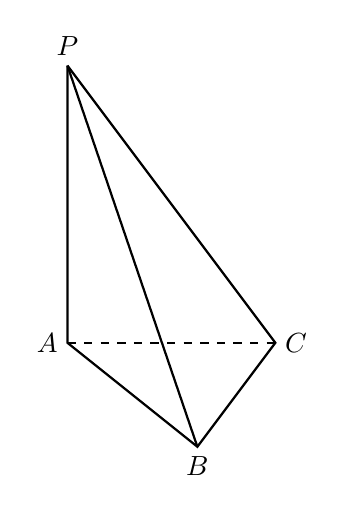
\begin{tikzpicture}[>=stealth, scale=1.1]
  % 顶点坐标
  \coordinate (A) at (0, 0);
  \coordinate (P) at (0, 3.2);
  \coordinate (C) at (2.4, 0);
  \coordinate (B) at (1.5, -1.2);

  % 实线棱
  \draw[thick] (P) -- (A) -- (B) -- (C) -- (P);
  \draw[thick] (P) -- (B);

  % 虚线棱
  \draw[dashed, thick] (A) -- (C);

  % 顶点标签
  \node[above] at (P) {$P$};
  \node[left] at (A) {$A$};
  \node[below] at (B) {$B$};
  \node[right] at (C) {$C$};
\end{tikzpicture}
